

\begin{figure}[h!]
    \centering
    \caption{Grade distribution}
    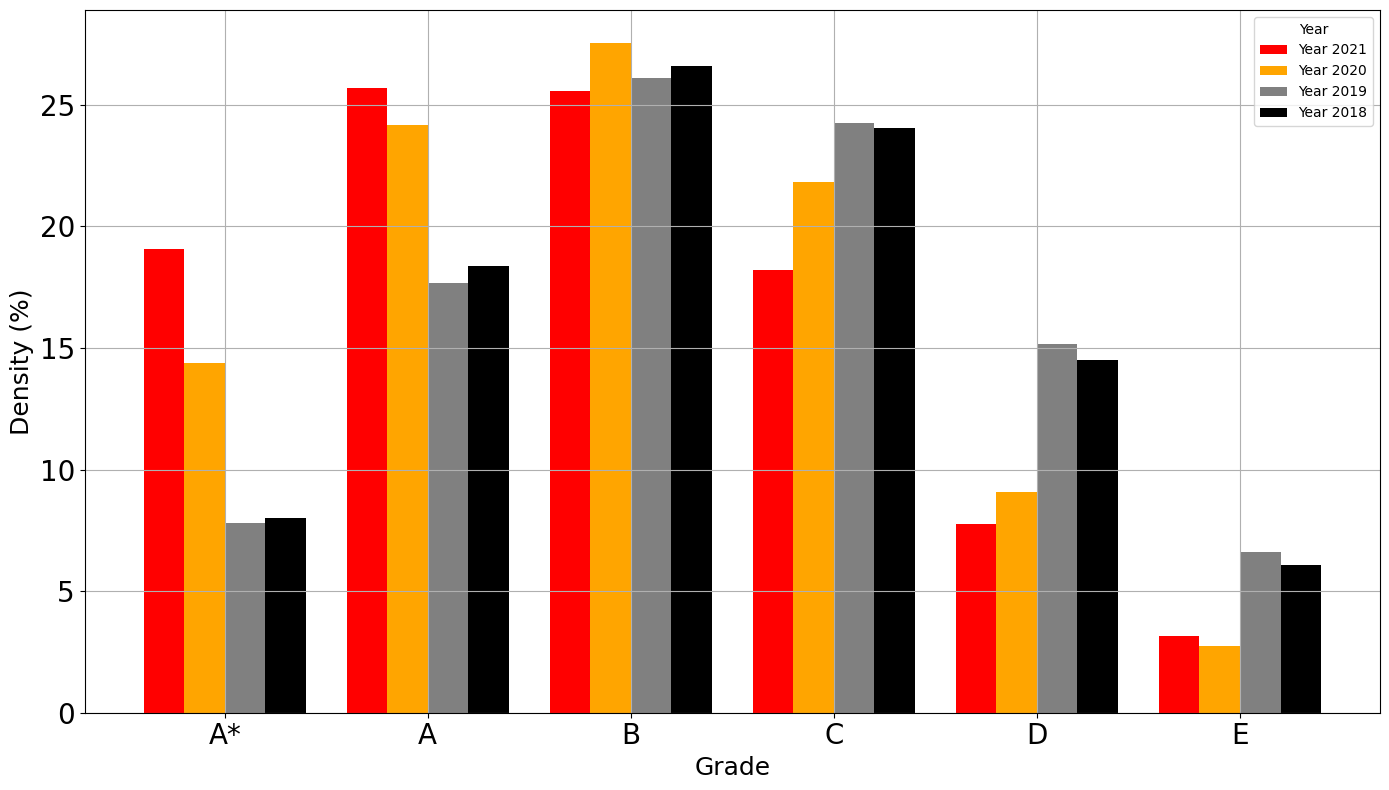
\includegraphics[width=\linewidth]{figures/Background/PDF_GradeInflation_Bar.png}
    \label{fig:grade_histogram}
      \caption*{\footnotesize Note: The histogram displays the share of letter grades issued for each grade bins in the A-levels between 2018 and 2021. A*,A denotes the highest grade assigned to exam results scoring above the top 90th and 80th percentile respectively. Sample is the universe of test takers in each year. Data is derived from grade reports from the Joint Councils of Qualifications.} 
\end{figure}
\clearpage


